%# -*- coding: utf-8-unix -*-
%%==================================================
%% chapter_4.tex for SJTU Master Thesis
%%==================================================

\chapter{时钟源漂移补偿的统计优化算法及统计策略在透明时钟的应用}
在第\ref{chap:statistical_delay}章中,本人从链路传输延时的角度,通过深入分析实际工业环境下对链路传输延时的影响,通过对链路传输延时建立细致的数学模型,并从数学统计的角度对其中各个影响因素提出了有针对性的解决方案。

至此,我们已经能够利用上述算法综合获得稳定和精确的链路延时。但是,仅仅获取稳定精确的链路延时并不是时钟同步的终点。想要提高同步精度意味着我们必须得出准确的主从偏差值offset,并对从时钟进行校正。但是,主从偏差值会由于晶振源频率波动而变化,所以依据常规的同步算法我们并不能消除这个问题。为了能够计算得到准确的offset,本人将采取的做法是对从时钟晶振频率进行补偿,从而使的主从时钟频率尽可能保持一致,从而消除offset波动所带来的问题。

另外,本章节还将介绍如何将稳中提到的统计算法应用到透明时钟中,由于透明时钟与边界时钟的根本差异,我们需要对统计算法进行调整才能更好的应用到透明时钟中。

最后,在现实IEEE1588协议运行中,之所以同步精度难以达到亚微秒的同步精度,有很重要的因素是从时钟校正策略的选取。所谓时钟同步,最核心一环自然是从时钟根据计算数据对本地进行校正来实现同步,即时钟伺服系统。所以在最后我们会简单探索下从时钟控制策略。常规我们在IEEE1588协议中采用的是PI控制策略,即利用PI控制器来对从时钟进行校正,而不是直接利用offset进行校正。这种做法能够一定程度提高从时钟的同步精度和稳定性,但它也存在如PI参数固定等缺陷而导致同步系统无法有效应对复杂多变的工业网络环境,这严重破坏了从时钟系统的鲁棒性和稳定性。因此,考虑到工业网络环境的复杂性和多变性,本文尝试从神经网络控制策略入手,以期待利用神经网络优秀的适应性来提高从时钟对复杂环境的鲁棒性和自适应性。

\section{主从时钟源频率漂移}
主从时钟源频率漂移
\subsection{从时钟频率补偿原理}
从时钟频率补偿原理
\subsection{统计算法在频率补偿中的应用}
统计算法在频率补偿中的应用

\section{统计算法在透明时钟中的应用}
透明时钟是一种新的ptp设备类型,虽然它应用范围不如边界时钟更广,而且其本身需要成本更高,不过为了算法完整性,本人还是决定对于这类设备的同步优化进行分析。下面的分析主要针对透明时钟与边界时钟的差异性,来分析四种算法暂时性时延抖动优化算法,持久性时延变化优化算法,时延固有波动优化算法和主从时钟源频率补偿算法的调整。

\subsection{透明时钟与边界时钟差异性}
透明时钟(Transparent Clock, TC)是1588v2中引入的一种新的ptp设备类型,它的基本原理是通过内部驻留时间桥来测量事件消息在通过设备时的驻留时间,然后把驻留时间存储到事件消息的修正域中。当从时钟接收到该报文时,可以通过解析修正域而得知该报文在链路传输过程中所经历的传输时间。

透明时钟有两种工作机制:
\begin{itemize}[noitemsep,topsep=0pt,parsep=0pt,partopsep=0pt]
  \item 端对端透明时钟(End to End TC)。这种工作机制下,透明时钟将转发所有符合网络规则的报文,同时测量出时间消息驻留时间,并把测量结果作为修正值累计啊到事件消息的修正域中;
  \item 点对点透明时钟(Peer to Peer TC)。这种工作机制下,透明时钟每个端口上额外添加一个延时测量模块,这个模块可以计算在该练路上,执行相同机制的对方端口之间的链路传输延时。所以说,点对点透明时钟不仅可以修正驻留时间,还能对端口之间的链路传输延时进行修正。不过,它只会对Sync报文和Followup报文进行处理,丢弃DelayReq和DelayResp报文。
\end{itemize}

依据上述透明时钟的原理,我们可以将其与边界时钟进行比较得到以下几个不同点:
\begin{itemize}[noitemsep,topsep=0pt,parsep=0pt,partopsep=0pt]
  \item 首先,边界时钟完全无法测量链路传输延时,而透明时钟可以计算在设备内部的驻留时间,因此,即使报文在传输过程中,遭遇排队或堵塞等暂时性时延波动,从时钟仍然能够通过减去修正域的值来消除其影响;
  \item 另外,假设链路发生了拓扑结构变化,所有报文的传输路径变动,我们依然可以利用透明时钟的特性消除因此带来的链路传输延时持久性变化。
\end{itemize}

\subsection{统计算法的调整与优化}
由于边界时钟与透明时钟的固有差异,如果我们想把上述的统计算法应用到透明时钟,则需要做出一些调整。而我们知道,透明时钟比边界时钟更高级,能够很好的衡量报文传输路径中消耗的延时,所以,如果我们在实际系统中采用了透明时钟,那么我们能够极大简化统计算法,也能够得到更好的同步精度。但是,目前工业应用中,透明时钟并没有完全替代边界时钟,一方面由于透明时钟成本更高,另一方面由于透明时钟的推出时间晚于边界时钟,工业中很多同步场合已经采用了边界时钟同步架构。

对于透明时钟,由于它能够较好的测量链路传输延时,那么我们可以作出以下调整:
\begin{itemize}[noitemsep,topsep=0pt,parsep=0pt,partopsep=0pt]
  \item 暂时性时延抖动算法:由于暂时性时延抖动主要源自中间设备内部的排队和堵塞,而透明时钟能够把这些时间添加到修正域中,因此即使设备发生排队现象,我们仍然能在从时钟处很好的消除这部分时间的变化,因此,如果一条链路中全部采用了透明时钟,那么可以不需要考虑此类时延抖动。不过,如果链路中同时采用了边界时钟与透明时钟,那么仍然有必要考虑算法实现;
  \item 持久性时延变化算法:所谓持久性时延变化主要来自于链路拓扑结构的变化,一旦链路变化,那么报文的链路传输时间则会发生变化,而对于统计算法而言,这也就意味着之前的统计样本统统失效。在透明时钟中,我们会减去设备内部的时间波动,那么只有纯粹链路的传输时间变化会导致样本的移动,不过,一般而言,纯粹路径耗时非常微小,所以可以当作持久性时延变化不会对透明时钟有很大影响;
  \item 时延固有波动算法:对于时延固有波动,无论透明时钟还是边界时钟都是无法消除的,所以,我们仍然要针对固有波动进行统计处理,以减小时延的波动造成从时钟源的波动,提高从时钟稳定性;
  \item 主从时钟源频率补偿算法:主从时钟源与中间传输设备没有太大关联,无论是边界时钟还是透明时钟,都需要进行频率补偿。只不过,由于该算法是利用Sync报文的发送周期与接收周期的差异来进行优化的,所以会受到Sync报文传输时间的影响,如果Sync报文路径传输时间变长,那么接收周期变大,导致计算出现偏差。所以,对于透明时钟而言,可以忽略报文传输的时间变化,因此透明时钟在频率补偿时会有更好的精度。
\end{itemize}

\section{时钟伺服系统研究}
对从时钟而言,如果想要实现与主时钟同步,就必须依靠前面提到的同步算法及所计算出来的链路时延值,从而对从时钟自身的相位和频率进行校正,以有效消除与主时钟之间的偏差。不过,由于当前的很多工业平台并非实时操作系统,所以一般而言都需要利用中断机制来触发从时钟进行校正。但是,在该中断过程中造成的从时钟漂移抖动会长期破坏同步精度,严重影响同步过程的实时性。

因此,为了提高从时钟校正过程的实时性和快速性,我们需要设计一套比较良好的时钟伺服系统来对从时钟进行校正。

\subsection{通用PTP时钟伺服系统介绍}
\begin{figure}[!hbp]
  \centering
  \begin{minipage}[b]{0.7\textwidth}
    \captionstyle{\centering}
    \centering
    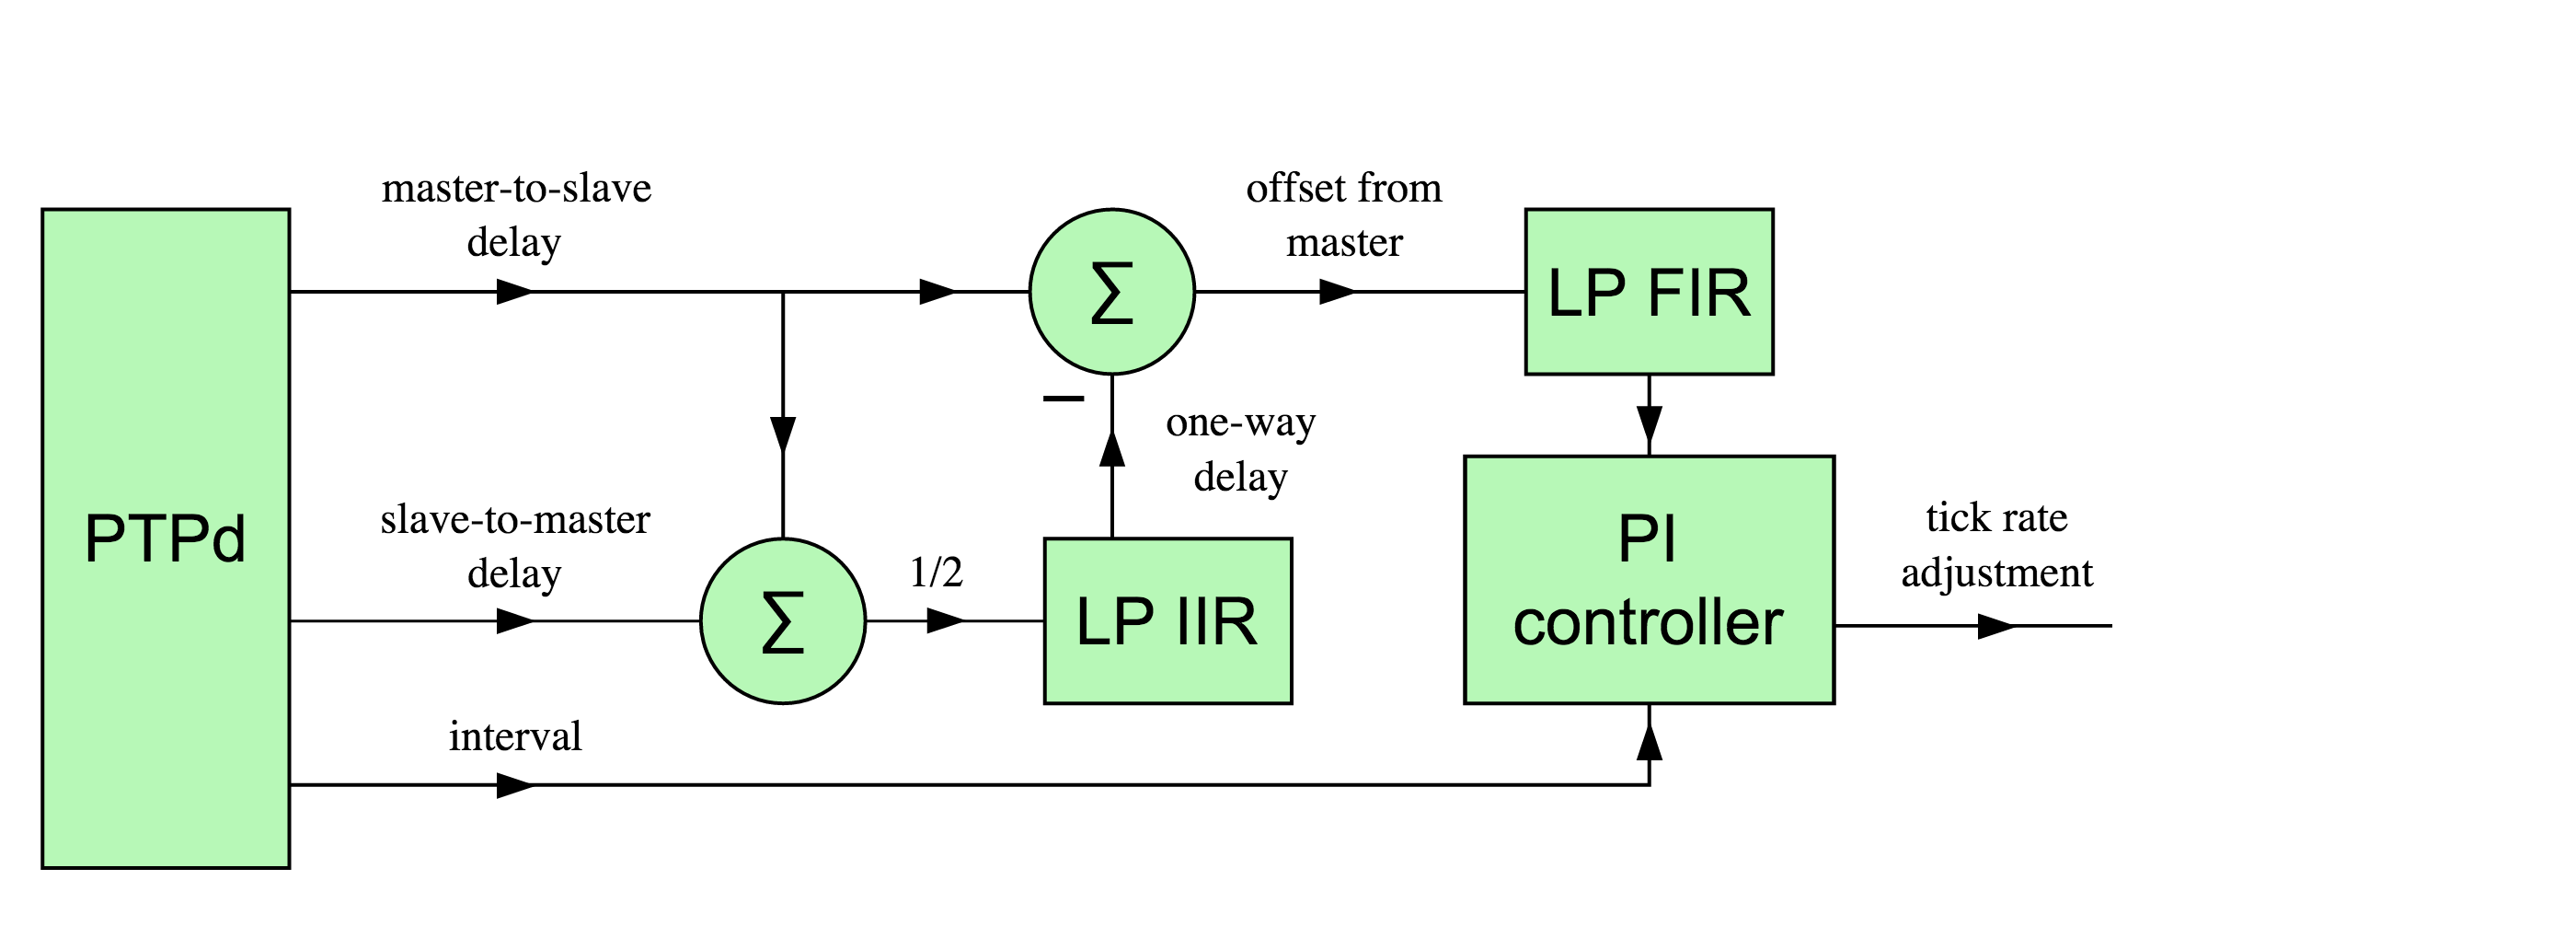
\includegraphics[width=11cm]{normal_clock_servo_system}
    \bicaption[fig:normal_clock_servo_system]{通用PTP时钟伺服系统}{通用PTP时钟伺服系统}{Fig}{The normal structure of general PTP clock servo system}
  \end{minipage}     
\end{figure}

一种常见的PTP时钟伺服系统如上图\ref{fig:normal_clock_servo_system}所示。从左到右表明了数据从PTP协议引擎逐渐流向从时钟。在该系统中,PTP协议引擎通过周期性获取主从偏差和从主偏差,将这两个偏差值通过均值滤波及低通滤波器获取到当前offset值。然后,将当前offset值与采样周期数据共同传递给PI控制器,由PI控制器来对从时钟进行校正以实现主从同步。该PI控制器由比例(P)和积分(I)两个环节共同构成,其中,比例环节可以用来消除主从时钟间的相位偏差,而积分项则可以用来消除系统的稳态误差,即消除主从时钟间的频率差\supercite{58}。

上述这样一套较为完整的时钟伺服系统可以较好的实现时钟同步,而且,由于传统的PI控制算法相对而言比较简单、鲁棒性良好且可靠性较高,所以传统的PI控制器在工业控制领域里应用十分广泛。

但是,传统的PI控制器也有其固有的弊病,那就是其比例积分参数的调整往往需要依靠经验来设定。对于处于复杂网络环境中的时钟同步系统而言,仅仅依靠经验来整定控制参数的PI控制器几乎无法应对任何形式的复杂多变的环境,尤其是同步系统中的网络环境中存在多种非线性、时变性等不确定性因素时,被控对象特性常常会随着时间发生变化。例如工业中充当从时钟的PTP设备,很容易会随着时间慢慢精度降低,并且长期受到工业干扰导致设备性能逐渐下降\supercite{59}。这些从时钟的变化都会导致传统的PI控制器在时钟伺服系统中无法达到良好的控制效果。

所以,为了使得时钟伺服系统能够适应工业网络环境变化,尤其是应对时变性非常强的网络传输环境,本人在下文从智能自适应控制的角度出发,结合同步系统特性进行深入分析,并且提出基于智能控制策略作为伺服系统中的控制环节,从而来弥补传统PI控制器无法适应复杂网络环境的缺陷。

\subsection{基于神经网络的PID控制策略}
根据上节可以知道,由于传统PI控制器无法适应网络传输环境和被控对象的时变性,我们需要采用一种能够自动根据当前网络环境而调整的控制策略。本人在此选择神经网络及PI控制相结合,以此来实现时钟伺服系统中对从时钟的控制。下文会对该控制策略进行详细讲解。

\subsection{神经网络介绍与研究}
神经网络作为模拟人的思维方式,它内部的单元多数都使用结构较为简单的神经元模型,然后通过对内部神经元之间的权值进行修正从而来实现对多维数据的非线性处理\supercite{61}。

\begin{figure}[!hbp]
  \centering
  \begin{minipage}[b]{0.6\textwidth}
    \captionstyle{\centering}
    \centering
    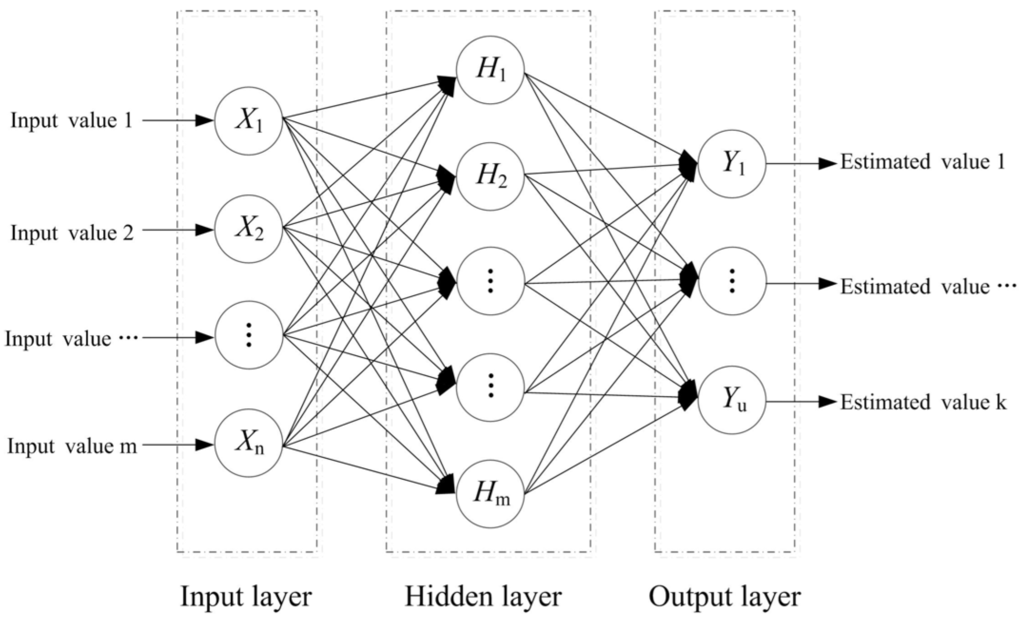
\includegraphics[width=10cm]{neural_network}
    \bicaption[fig:neural_network]{神经网络结构图}{神经网络结构图}{Fig}{The structure of neural network}
  \end{minipage}     
\end{figure}

根据图\ref{fig:neural_network}可以看到神经网络的整体结构,在一套完整的神经网络结构中,一般会包含多个不同的网络层单元,即下列几个网络层:
\begin{itemize}[noitemsep,topsep=0pt,parsep=0pt,partopsep=0pt]
	\item 输入层(Input Layer):这一层的输入节点主要接收外部数据的特征变量。对于这些特征变量的选取,必须能够准确地描述外界事物,依据选择对象的特征来选择有意义的原始特征变量,这也称为特征空间。所以说,这一层中会有大量神经元接受外界复杂的非线性输入信息。
	\item 隐含层(Hidden Layer):这一层是中间层,即位于输入层与输出层之间的一层,包含众多神经元和链接。事实是隐含层可以有多层,但习惯上我们只会用一层。这一层的节点数目不定,但数目越多的话,对应的网络非线性越显著,使得神经网络的强健性更为明显\footnote{强健性即控制系统在一定结构、大小等的参数摄动下,维持某些性能的特性。}。一般而言可以选输入节点数1.2至1.5倍的节点。
	\item 输出层(Output Layer):这一层是神经网络经过计算后将计算值对外输出的一层。所有原始数据在神经元节点中进行传输、分析,最终形成输出结果,我们把输出的信息结果数据称为输出向量。
\end{itemize}

\subsection{神经网络与时钟伺服系统的关联性研究}
之所以本文会采取神经网络作为时钟伺服的控制学习策略,主要基于以下几点考虑:
\begin{itemize}[noitemsep,topsep=0pt,parsep=0pt,partopsep=0pt]
	\item 神经网络是高度非线性动力学系统,又是自适应自组织系统,而我们的时钟同步系统所在的工业网络环境也是非常复杂且时变的,所以,我们需要一个学习策略能够根据外界网络环境的变化来调节自身,具备良好自适应性\supercite{64}。因此,神经网络是一个很好的选择。
	\item 神经网络具备学习功能,即通过学习大量的样本数据来获取输入输出之间的函数关系,这对于数学模型复杂或难以建立的系统具备良好的适应性,而我们的从时钟系统便由于工业现场的多变性而难以建立准确的数学模型。因此,神经网络能够发挥样本数据的优势来解决。
	\item 神经网络是一种数据非线性映射工具,相对于传统统计的数学方法而言,不仅不会产生冲突,而且可以互相补充\supercite{68}。由上文介绍知道,本文中采用了多种数学统计方法,也积累了很多样本数据,因此,数学统计策略与神经网络模型可以良好的结合在一起。
\end{itemize}

因此,由于神经网络高度的自学习能力,非常适合模拟复杂的非线性系统。根据神经网络理论中的Kolmogorov连续性定理,给定任一连续函数
\begin{align}
f:[0,1] \quad n \rightarrow Rm
\end{align}
f,我们都可以用一个三层前馈神经网络来精确地实现,从数学上保证了神经网络用语时间序列预测的可行性。而且,本文中采用了多种数学统计方法,积累了很多的样本数据,而神经网络作为数据非线性映射工具,可以和前面所提的数学统计方法得到非常良好的结合。

\subsection{基于BP神经网络的PID控制策略实现}
由上文可知,对于时钟同步系统而言,由于工业网络环境复杂且时刻变化,简单的PI控制完全无法应对多变的环境,也不具备任何自适应性。所以,仅仅采用简单的PI控制无法使的从时钟系统能够达到很好的稳定性和收敛性,甚至可能由于网络环境的不断变化而发生振荡甚至难以稳定。因此,一种能够控制非线性且时变的对象的控制策略对于工业环境下时钟同步系统而言至关重要。

在上一小节中,本人通过对神经网络基础原理及相关理论进行了较为深入的研究。可以看出,神经网络算法不仅具备良好的学习功能,这能帮助从时钟在复杂的网络环境下不断对自身进行调整以达到良好的同步效果,而且,该算法作为数据非线性映射工具,还能与传统统计方法相互补充,而本人在前面已经采取了多种统计算法,所以,在从时钟端会累积很多样本数据,这些样本的存在正好使的神经网络算法发挥更大的作用\supercite{63}。

为了将神经网络算法应用于时钟伺服系统中,我们可以将神经网络与PID控制系统相结合,通过外界输入样本对神经网络进行训练,然后让神经网络对外输出PID控制系统所需要的三种控制参数$K_{i}$、$K_{p}$、$K_{d}$。可以参考下图的结构设计:

\begin{figure}[!hbp]
  \centering
  \begin{minipage}[b]{0.6\textwidth}
    \captionstyle{\centering}
    \centering
    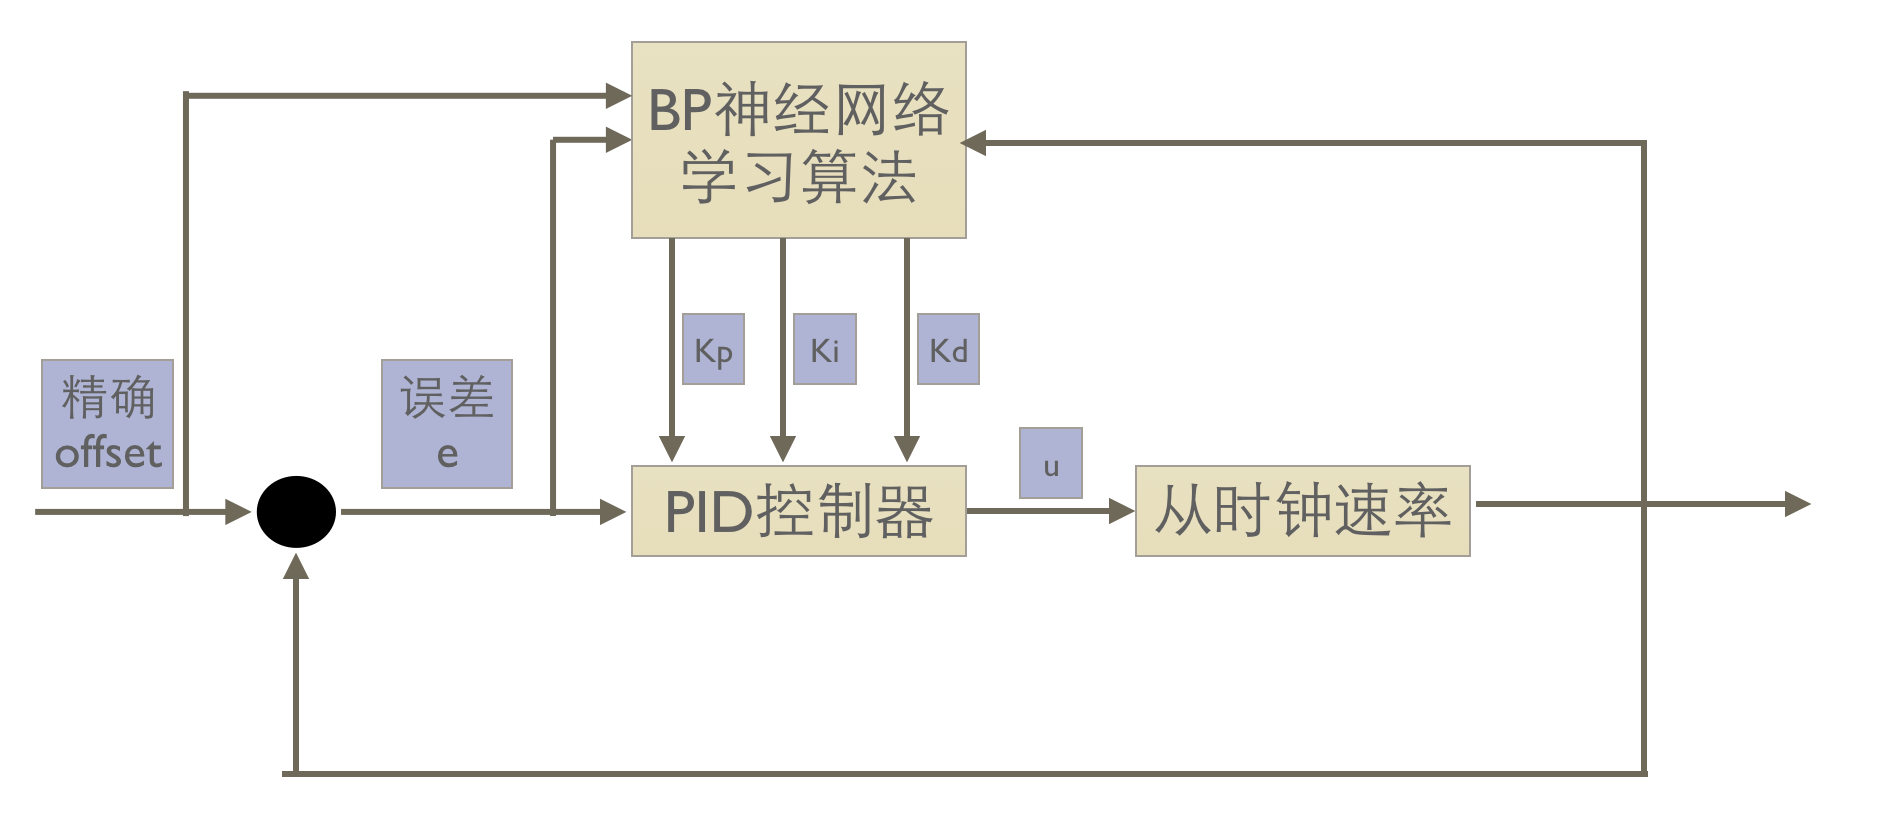
\includegraphics[width=10cm]{bp_neural_network_PID}
    \bicaption[fig:bp_neural_network_PID]{基于BP神经网络的PID控制系统结构图}{基于BP神经网络的PID控制系统结构图}{Fig}{The structure combining BP neural network with PID controller}
  \end{minipage}     
\end{figure}

\subsubsection{BP神经网络结构}
下图\ref{fig:bp_neural_network}为BP\footnote{Back Propagation 误差反向传播}神经网络结构图,从左往右依次为输入层、隐含层、输出层,下文将依据该结构,将伺服系统分成前向传播过程和误差反向传播过程来分别讲述。
\begin{figure}[!hbp]
  \centering
  \begin{minipage}[b]{0.6\textwidth}
    \captionstyle{\centering}
    \centering
    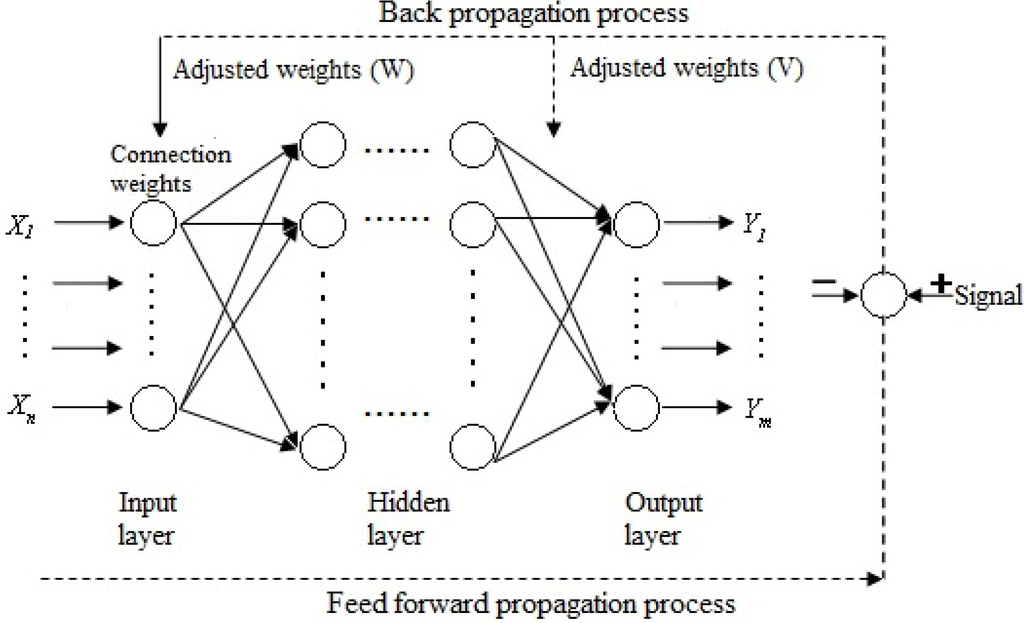
\includegraphics[width=10cm]{BP_neural_network}
    \bicaption[fig:bp_neural_network]{BP神经网络结构图}{BP神经网络结构图}{Fig}{The structure of BP neural network}
  \end{minipage}     
\end{figure}

\subsubsection{前向计算过程}
该过程是指输入变量依次经过输入层、隐含层直到输出层的过程。首先,对于输入层,我们可以选取k个主从偏差样本作为神经网络的输入。该样本个数k若太大,则会导致训练时间过长,系统需要较长时间的收敛过程;反之,若样本个数$K_{i}$太小,则会导致达不到学习效果\supercite{69}。在此,本人将$K_{i}$选取为4。所以,输入层的输入为:
\begin{align}
	input_{1} = offset_{c}, input_{2} = offset_{(c-1)}, \\
	input_{3} = offset_{(c-2)}, input_{4} = offset_{(c-3)}, 
\end{align}
其中,$offset_{c}$是表示当前时刻计算得到的时延值。所以,在输入层第i个输入节点的输出值为:
\begin{align}
	InputLayer\_Output_{i} = input_{i} \qquad i = 1, 2, 3, 4
\end{align}

然后,在隐含层有$K_{h}$个神经元节点,那么假设对于隐含层的第j个神经元的输入为:
\begin{align}
	HiddenLayer\_Input_{j} = \sum_{j=1}^{K_{h}}(W_{ij}InputLayer\_Output_{i})
\end{align}
即每一个隐含层节点的输入为所有输入层节点输出值乘以权值的总和。我们可以得到其隐含层节点的输出值为:
\begin{align}
	HiddenLayer\_Output_{j} = f(HiddenLayer\_Input_{j}) \qquad j = 1, 2 \cdots K_{h}
\end{align}

最后,在输出层,我们只选取三个输出节点,这三个节点分别对外提供三个控制参数$K_{i}$、$K_{p}$、$K_{d}$。
\begin{align}
K_{o} = 3
\end{align}
对于其中第z个输出节点,可以得到其输入值为:
\begin{align}
OutputLayer\_Input_{z} = \sum_{j=1}^{K_{h}}(W_{jz}HiddenLayer\_Output_{j}) \qquad z = 1, 2, 3
\end{align}
同时,我们可以得到第z个输出节点的最终输出值为:
\begin{align}
OutputLayer\_Output_{z} = g(HiddenLayer\_Input_{j}) \qquad j = 1, 2 \cdots K_{o}
\end{align}
其中,我们依次取各个输出为如下对应控制参数:
\begin{align}
K_{p} = OutputLayer\_Output_{1}
K_{i} = OutputLayer\_Output_{2}
K_{d} = OutputLayer\_Output_{3}
\end{align}

在上面的几个方程中,我们用$W_{ij}$来表示输入层到隐含层加权系数,然后用$W_{jz}$来表示隐含层到输出层的加权系数。另外,对于活化函数有多种选择方式,本人对于输入层\-隐含层及隐含层\-输出层分别取下面两个活化函数:
\begin{align}
Log-Sigmoid : f(x) = \frac{1}{1 + e^{-x}} \\
Sigmoid : g(x) = \frac{e^{x} - e^{-x}}{e^{x} + e^{-x}}
\end{align}

至此,我们已经可以从输出层得到三个控制参数$K_{i}$、$K_{p}$、$K_{d}$。但是,目前得到的三个控制参数并不能保证系统稳定,我们还需要误差反向传播过程,将实际误差反向传回给神经网络,并依靠该误差来进行加权系数的校正。

\subsubsection{误差反向传播}
根据上文中,我们已经了解到了BP神经网络算法中的固有缺陷,同时本人已经在上文中介绍响应的改进算法,下面,我们就该增加动量法来进行反向传播调节的实际。

首先,我们依据最速下降法取性能指标函数为:
\begin{align}
T(k) = \frac{1}{2}(Rin(k) - Yout(k))^{2}
\end{align}
同时,我们利用近似最速下降法来更新该系统中的各个权值,具体的更新方法如下:
\begin{align}
\Delta W_{jz}(k) = -\eta \frac{\partial E(k)}{\partial W_{jz}} + \alpha \Delta W_{jz}(k-1)
\end{align}
在上式子中,$\alpha$用来表示惯性系数,$\eta$用来表示学习速度,式子的后半部分是指在k-1时刻网络权值的修改方向,这也正是上文中所介绍的增加动量法的权值更新方式。也就是说,如果第k次的更新方向与k-1次相同,那么后半部分就为正,从而加速整个更新过程,相反,如果二者方向不同,那么后半部分为负,从而起到稳定更新算法的作用。

\subsubsection{基于离线BP神经网络的PID控制策略小结}
利用上述基于BP神经网络的PID控制器,通过神经网络与输入样本值来计算控制器所需的三个控制参数,从而实现对从时钟的校正。在下文中,我们会对这种方法的效果进行仿真,结合该结果我们可以看出,采用离线神经网络训练后的PID控制器可以起到不错的优化效果,在一定程度上能提高时钟伺服系统的稳定性和适应性。

但是,我们也能发现其中仍然存在的缺陷。一般而言神经网络需要一定的训练时间,对于资源非常有限的交换机设备而言,在线进行神经网络训练目前而言是不够现实的。所以,我们只能采用离线训练的方法,来降低该方法对交换机本身的负载压力。因此,这势必会导致神经网络的实时性有所缺陷,即不能实时利用采集样本数据来进行训练。

因此,离线BP神经网络由于其能采用实际的时延样本来进行训练,所以能够取得不错的鲁棒性和自适应性。这是其他方法,例如常规PI控制策略所不具备的,它所能带来的高稳定性和高鲁棒性也是对高精度时钟同步系统而言非常需要的。但是,我们也应该明确这种方法存在的固有漏洞,那就是神经网络方法本身会需要较多的计算资源和空间资源,才能取得良好的效果。根据当前的应用实践,本人认为离线BP神经网络是目前而言具备良好的应用价值的。未来随着交换机等设备的升级和对时钟精度的更高要求,或许有可能在上面使用在线BP神经网络来进一步改善鲁棒性和自适应性。







